\ifx\pdfminorversion\undefined\else\pdfminorversion=4\fi
\documentclass[aspectratio=169,t]{beamer}
%\documentclass[aspectratio=169,t,handout]{beamer}

% English version FAU Logo
\usepackage[english]{babel}
% German version FAU Logo
%\usepackage[ngerman]{babel}

\usepackage[utf8]{inputenc}
\usepackage[T1]{fontenc}
\usepackage{amsmath,amssymb}
\usepackage{graphicx}
\usepackage{listings}
\usepackage{url}
\usepackage{hyperref}
\usepackage{fontawesome}
\usepackage{tikz}
\usepackage{tikz-cd}

\tikzset{
    vertex/.style = {
        circle,
        fill            = black,
        outer sep = 2pt,
        inner sep = 1pt,
    }
}
\usetikzlibrary{matrix,mindmap}
\usetikzlibrary{arrows,decorations.pathmorphing,backgrounds,fit,positioning,shapes.symbols,chains,intersections}
\tikzset{level 1/.append style={sibling angle=50,level distance = 165mm}}
\tikzset{level 2/.append style={sibling angle=20,level distance = 45mm}}
\tikzset{every node/.append style={scale=1}}
% Options:
%  - inst:      Institute
%                 med:      MedFak FAU theme
%                 nat:      NatFak FAU theme
%                 phil:     PhilFak FAU theme
%                 rw:       RWFak FAU theme
%                 rw-jura:  RWFak FB Jura FAU theme
%                 rw-wiso:  RWFak FB WISO FAU theme
%                 tf:       TechFak FAU theme
%  - image:     Cover image on title page
%  - plain:     Plain title page
%  - longtitle: Title page layout for long title
\usetheme[%
  image,%
  longtitle,%
  tf
]{fau}

% Enable semi-transparent animation preview
\setbeamercovered{transparent}


\lstset{%
  language=Python,
  tabsize=2,
  basicstyle=\tt,
  keywordstyle=\color{blue},
  commentstyle=\color{green!50!black},
  stringstyle=\color{red},
  numbers=left,
  numbersep=0.5em,
  xleftmargin=1em,
  numberstyle=\tt
}


% Title, authors, and date
\title[KDD]{Chapter I: Introduction}
\subtitle{Knowledge Discovery in Databases}
\author[L.~Melodia]{Luciano Melodia M.A.}
% English version
\institute[Department]{Evolutionary Data Management, Friedrich-Alexander University Erlangen-Nürnberg}
% German version
%\institute[Lehrstuhl]{Lehrstuhl, Friedrich-Alexander-Universit\"at Erlangen-N\"urnberg}
\date{Summer semester 2021}
% Set additional logo (overwrites FAU seal)
%\logo{\includegraphics[width=.15\textwidth]{themefau/art/xxx/xxx.pdf}}


\begin{document}
  % Title
  \maketitle

  {
    \setbeamertemplate{footline}[frame number]
    \begin{frame}{Chapter I: Introduction}
    This is our agenda for this lecture:
        \begin{itemize}
            \item \textbf{Why data mining?}
            \item What is data mining?
            \item A multi-dimensional view of data mining.
            \item What kind of data can be mined?
            \item What kinds of patterns can be mined?
            \item What technologies are used?
            \item What kinds of applications are targeted?
            \item Major issues in data mining.
            \item A brief history of data mining.
            \item Summary.
        \end{itemize}
    \end{frame}
  }

  {
    \setbeamertemplate{footline}[frame number]
    \begin{frame}{Why Data Mining?}
    \textbf{The explosive growth of data: from terabytes to petabytes and more.}\\
        \begin{itemize}
            \item Data collection and availability:
                \begin{itemize}
                    \item Automated data collection tools.
                    \item Database systems.
                    \item World wide web.
                    \item Computerized society.
                    \item Digitization.
                \end{itemize}
            \item Major sources of abundant data:
                \begin{itemize}
                    \item Business: web, e-commerce, transactions, stocks \ldots
                    \item Science: remote sensing, bioinformatics, scientific simulation \ldots
                    \item Society: news, digital cameras, social media \ldots
                \end{itemize}
            \item The era of \textbf{big data} (as inflationary used buzzword).
        \end{itemize}
    \textbf{We are drowning in data, but starving for knowledge.} \textbf{Necessity is the mother of invention.}\\
    For data mining it is the automated analysis of massive data sets.
    \end{frame}
  }

  {
    \setbeamertemplate{footline}[frame number]
    \begin{frame}{Evolution of Sciences (I)}
        \begin{itemize}
            \item Before $1600$, era of \textbf{empirical science}.
            \item $1600-1950$s, rise of \textbf{theoretical science}.
                  \begin{itemize}
                      \item Each discipline has grown a theoretical component.
                      \item Theoretical models often motivate experiments and generalize our understanding.
                  \end{itemize}
            \item $1950-1990$s, rise of \textbf{computational science}.
                  \begin{itemize}
                      \item Over the last $50$ years most disciplines have grown a third, computational branch.
                      \begin{itemize}
                          \item E.g. empirical, theoretical and computational ecology.
                          \item E.g. physics, linguistics or biology.
                      \end{itemize}
                  \end{itemize}
            \item Computational science traditionally meant simulation.
            \item It grew out of our inability to describe reality by closed-form mathematical models.
        \end{itemize}
    \end{frame}
  }

  {
    \setbeamertemplate{footline}[frame number]
    \begin{frame}{Evolution of Sciences (II)}
        \begin{itemize}
            \item $1990-$now, rise of \textbf{data science}.
                  \begin{itemize}
                      \item The flood of data from new instruments and modern simulations.
                      \item The ability to economically store and manage petabytes of data.
                      \item The internet makes all these archives world wide accessible.
                      \item Scientific \emph{information management}, \\
                            acquisition,\\
                            organization, \\
                            query and \\
                            visualization scale almost linearly with amount of data.
                      \item \textbf{Data mining} is a major new challenge!
                  \end{itemize}
          \item For further reading:\\
                \small{Jim Gray and Alex Szaly: \emph{The World Wide Telescope: An Archetype for Online Science}, \\ Communications of the ACM 45(11): 50-54, 2002.}
        \end{itemize}
    \end{frame}
  }

  {
    \setbeamertemplate{footline}[frame number]
    \begin{frame}{Evolution of Sciences (III)}
        \begin{itemize}
            \item $1960$s: Data collection, \\
                  \hspace{1cm} database creation, \\
                  \hspace{1cm} integrated management systems (IMS) and \\
                  \hspace{1cm} network database management systems (DBMS).
            \item $1970$s: Relational data model, relational DBMS implementation (RDBMS).
            \item $1980$s: RDBMS products,\\
                  \hspace{1cm} database creation, \\
                  \hspace{1cm} advanced data models (extended relational, object oriented, deductive etc.),\\
                  \hspace{1cm} application-oriented DBMS (spatial, scientific, engineering etc.).
            \item $1990$s: Data mining,\\
                  \hspace{1cm} data warehousing, \\
                  \hspace{1cm} multimedia databases,\\
                  \hspace{1cm} web databases.
            \item $2000$s: Stream data management and mining,\\
                  \hspace{1cm} data mining and applications, \\
                  \hspace{1cm} web technology (XML, data integration) and global information systems.
        \end{itemize}
    \end{frame}
  }

  {
    \setbeamertemplate{footline}[frame number]
    \begin{frame}{Chapter I: What is Data Mining?}
        \begin{itemize}
            \item Why data mining?
            \item \textbf{What is data mining?}
            \item A multi-dimensional view of data mining.
            \item What kind of data can be mined?
            \item What kinds of patterns can be mined?
            \item What technologies are used?
            \item What kinds of applications are targeted?
            \item Major issues in data mining.
            \item A brief history of data mining.
            \item Summary.
        \end{itemize}
    \end{frame}
  }

  {
    \setbeamertemplate{footline}[frame number]
    \begin{frame}{What is Data Mining?}
    \textbf{Data mining or knowledge discovery from data}:
        \begin{itemize}
            \item Extraction of interesting (\textbf{non-trivial, implicit, previously unknown \\
                  and potentially useful}) patterns from huge amounts of data.
            \item Is \textbf{data mining} a misnomer?
        \end{itemize}
    Alternative names:
        \begin{itemize}
            \item Knowledge discovery/mining in databases (KDD).
            \item Knowledge extraction.
            \item Data/pattern analysis.
            \item Data archeology.
            \item Data dredging.
            \item Information harvesting.
            \item Business intelligence.
        \end{itemize}
    Watch out: Is everything \textbf{data mining}?
        \begin{itemize}
            \item Simple search and query processing is considered not to be.
            \item Neither are deductive expert systems.
        \end{itemize}
    \end{frame}
  }


  {
    \setbeamertemplate{footline}[frame number]
    \begin{frame}{Knowledge Discovery Pipeline}
    \begin{itemize}
        \item This is a typical view from a typical database-systems and data-warehousing community.
        \item Data mining plays an essential role in the knowledge-discovery process.
    \end{itemize}

    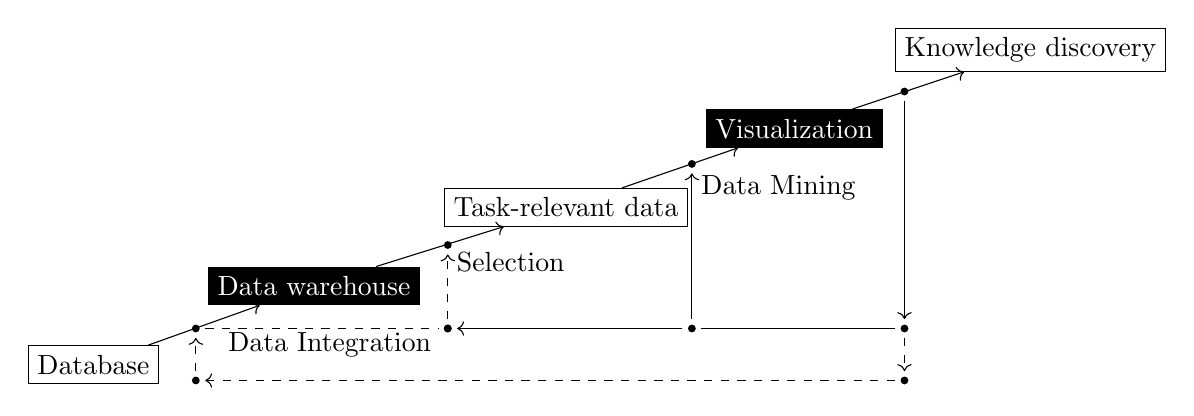
\begin{tikzpicture}
      % Dialectics
      \node[draw] (Database) at (0,0) {Database};
      \node[draw,fill=black,text=white] (Data warehouse) at (2.8,1) {Data warehouse};
      \node[draw] (Task-relevant data) at (6,2) {Task-relevant data};
      \node[draw,fill=black,text=white] (Data mining) at (8.9,3) {Visualization};
      \node[draw] (Knowledge discovery) at (11.9,4) {Knowledge discovery};

      \node (Data Integration) at (3,0.25) {Data Integration};
      \node (Selection) at (5.3,1.3) {Selection};
      \node (Data Mining) at (8.7,2.25) {Data Mining};

      \draw node[vertex] (Joint1) at (1.3,0.46) {};
      \draw node[vertex] (Joint2) at (4.5,1.52) {};

      \draw node[vertex] (Joint3) at (4.5,0.46) {};
      \draw node[vertex] (Joint7) at (4.5,0.46) {};
      \draw node[vertex] (Joint8) at (7.6,0.46) {};
      \draw node[vertex] (Joint9) at (10.3,0.46) {};
      \draw node[vertex] (Joint10) at (10.3,-0.2) {};
      \draw node[vertex] (Joint11) at (1.3,-0.2) {};

      \draw node[vertex] (Joint5) at (7.6,2.55) {};
      \draw node[vertex] (Joint6) at (10.3,3.47) {};


      \draw[->,draw=black] (Database) to (Data warehouse);
      \draw[->,draw=black] (Data warehouse) to (Task-relevant data);
      \draw[->,draw=black] (Task-relevant data) to (Data mining);
      \draw[->,draw=black] (Data mining) to (Knowledge discovery);
      \draw[-,draw=black, dashed] (Joint1) to (Joint3);
      \draw[->,draw=black, dashed] (Joint3) to (Joint2);
      \draw[->,draw=black] (Joint6) to (Joint9);
      \draw[-,draw=black] (Joint9) to (Joint8);
      \draw[->,draw=black] (Joint8) to (Joint7);
      \draw[->,draw=black] (Joint8) to (Joint5);
      \draw[->,draw=black,dashed] (Joint10) to (Joint11);
      \draw[->,draw=black,dashed] (Joint9) to (Joint10);
      \draw[->,draw=black,dashed] (Joint11) to (Joint1);
      \end{tikzpicture}
    \end{frame}
  }

   {
    \setbeamertemplate{footline}[frame number]
    \begin{frame}{Example: A Web-mining Framework}
    \textbf{Web mining usually involves:}
    \begin{itemize}
        \item Data cleaning.
        \item Data integration from multiple sources.
        \item Warehousing the data.
        \item Data-cube construction.
        \item Data selection for data mining.
        \item Data mining.
        \item Presentation of the mining results.
        \item Patterns and knowledge to be used or stored in a knowledge base.
    \end{itemize}
    \end{frame}
  }

  {
    \setbeamertemplate{footline}[frame number]
    \begin{frame}{Data Mining in Business}
    \centering
    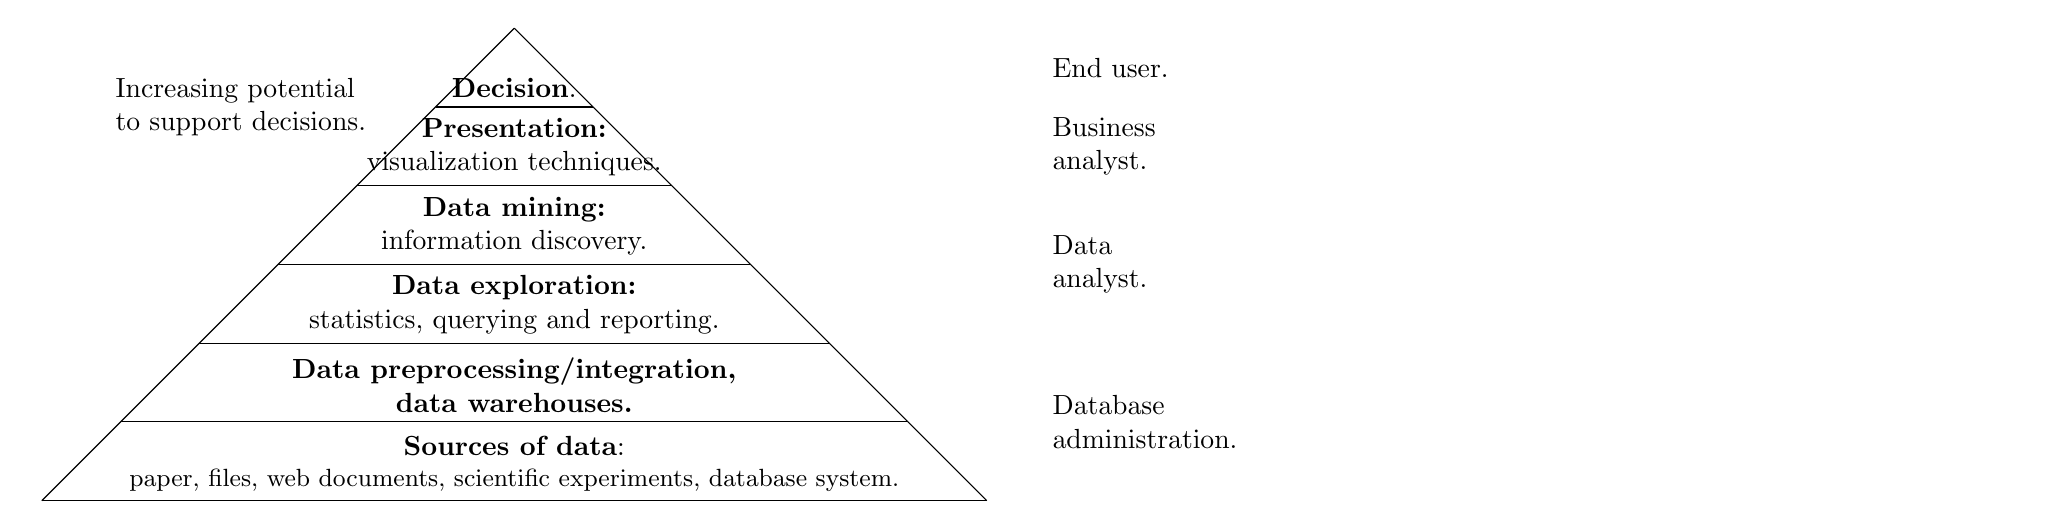
\begin{tikzpicture}
    \coordinate (A) at (-6,0) {};
    \coordinate (B) at ( 6,0) {};
    \coordinate (C) at (0,6) {};
    \draw[name path=AC] (A) -- (C);
    \draw[name path=BC] (B) -- (C);

    \node (Data Integration) at (1,5) {\parbox{\linewidth}{Increasing potential \\ to support decisions.}};
    \node (Data Integration) at (12.9,1) {\parbox{\linewidth}{Database \\ administration.}};
    \node (Data Integration) at (12.9,3) {\parbox{\linewidth}{Data \\ analyst.}};
    \node (Data Integration) at (12.9,4.5) {\parbox{\linewidth}{Business \\ analyst.}};
    \node (Data Integration) at (12.9,5.5) {\parbox{\linewidth}{End user.}};

    \foreach \y/\A in {0/{
        \parbox{\linewidth}{\centering \textbf{Sources of data}: \\ \small{paper, files, web documents, scientific experiments, database system.}}},
        1/\parbox{\linewidth}{\centering \textbf{Data preprocessing/integration,\\ data warehouses.}},
        2/\parbox{\linewidth}{\centering \textbf{Data exploration:} \\ statistics, querying and reporting.},
        3/\parbox{\linewidth}{\centering \textbf{Data mining:} \\ information discovery.},
        4/\parbox{\linewidth}{\centering \textbf{Presentation:} \\ visualization techniques.},
        5/\parbox{\linewidth}{\centering \textbf{Decision}.}} {
        \path[name path=horiz] (A|-0,\y) -- (B|-0,\y);
        \draw[name intersections={of=AC and horiz,by=P},
              name intersections={of=BC and horiz,by=Q}] (P) -- (Q)
            node[midway,above] {\A};
    }
    \end{tikzpicture}
    \end{frame}
  }

  {
    \setbeamertemplate{footline}[frame number]
    \begin{frame}{Example: Mining vs. Data Exploration}
    \begin{itemize}
        \item Business intelligence view:
        \begin{itemize}
            \item Warehouse, data cube or reporting.
            \item But not much mining.
        \end{itemize}
        \item Business objects vs. data mining tools.
        \item Supply chain example: tools.
        \item Data presentation.
        \item Exploration.
    \end{itemize}
    \end{frame}
  }

  {
    \setbeamertemplate{footline}[frame number]
    \begin{frame}{KDD Pipeline: A Typical View from Machine Learning and Statistics}
    \begin{itemize}
        \item This is a view from typical machine-learning and statistics communities.
    \end{itemize}
    \vspace{0.5cm}
    \centering
    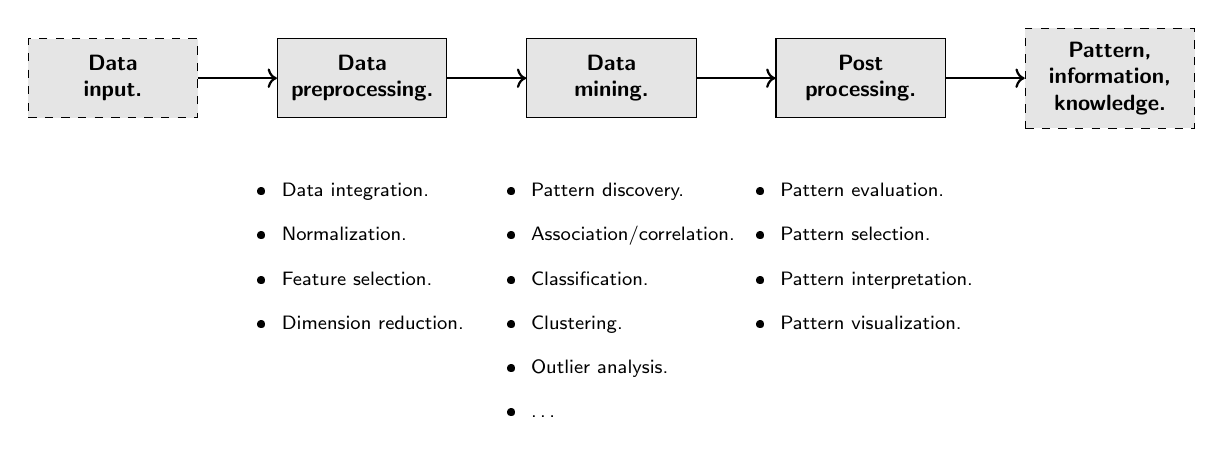
\begin{tikzpicture}
    [node distance = 1cm, auto,font=\footnotesize,
    % STYLES
    every node/.style={node distance=1cm},
    % The comment style is used to describe the characteristics of each force
    comment/.style={rectangle, inner sep= 5pt, text width=3.8cm, node distance=0.5cm, font=\scriptsize\sffamily},
    % The force style is used to draw the forces' name
    force/.style={rectangle, draw, fill=black!10, inner sep=5pt, text width=1.8cm, text badly centered, minimum height=1cm, font=\bfseries\footnotesize\sffamily}]

    % Draw forces
    \node [force, dashed] (a) {\parbox{\linewidth}{\centering Data \\ input.}};
    \node [force, right=1cm of a] (b) {\parbox{\linewidth}{\centering Data \\ preprocessing.}};
    \node [force, right=1cm of b] (c) {\parbox{\linewidth}{\centering Data \\ mining.}};
    \node [force, right=1cm of c] (d) {\parbox{\linewidth}{\centering Post \\ processing.}};
    \node [force, dashed, right=1cm of d] (e) {\parbox{\linewidth}{\centering Pattern, \\ information, \\ knowledge.}};

    %%%%%%%%%%%%%%%
    % Change data from here

    % SUPPLIERS
    \node [comment, below=0.25cm of b] {
    \begin{itemize}
        \item Data integration.
        \item Normalization.
        \item Feature selection.
        \item Dimension reduction.
    \end{itemize}
    };

    % USERS
    \node [comment, below=0.25 of c] {
    \begin{itemize}
        \item Pattern discovery.
        \item Association/correlation.
        \item Classification.
        \item Clustering.
        \item Outlier analysis.
        \item \ldots
    \end{itemize}
    };

    % PUBLIC POLICIES
    \node [comment, below=0.25 of d] {
      \begin{itemize}
        \item Pattern evaluation.
        \item Pattern selection.
        \item Pattern interpretation.
        \item Pattern visualization.
    \end{itemize}
    };

    \path[->,thick]
    (a) edge (b)
    (b) edge (c)
    (c) edge (d)
    (d) edge (e);

    \end{tikzpicture}
    \end{frame}
  }

  {
    \setbeamertemplate{footline}[frame number]
    \begin{frame}{Example: Medical Data Mining}
    \begin{itemize}
        \item \textbf{Health care and medical data mining}:
        \begin{itemize}
            \item Often adopted such a view in statistics and machine learning.
        \end{itemize}
        \item \textbf{Preprocessing of data}:
        \begin{itemize}
            \item Includes feature extraction and dimension reduction.
        \end{itemize}
        \item \textbf{Classification and/or clustering processes.}
        \item \textbf{Post processing for presentation}.
    \end{itemize}
    \end{frame}
  }

 {
    \setbeamertemplate{footline}[frame number]
    \begin{frame}{CRISP-DM}
    \begin{itemize}
        \item \textbf{CRoss-Industry Standard Process for Data Mining}:
    \end{itemize}
      \vspace{0.5cm}
    \centering
    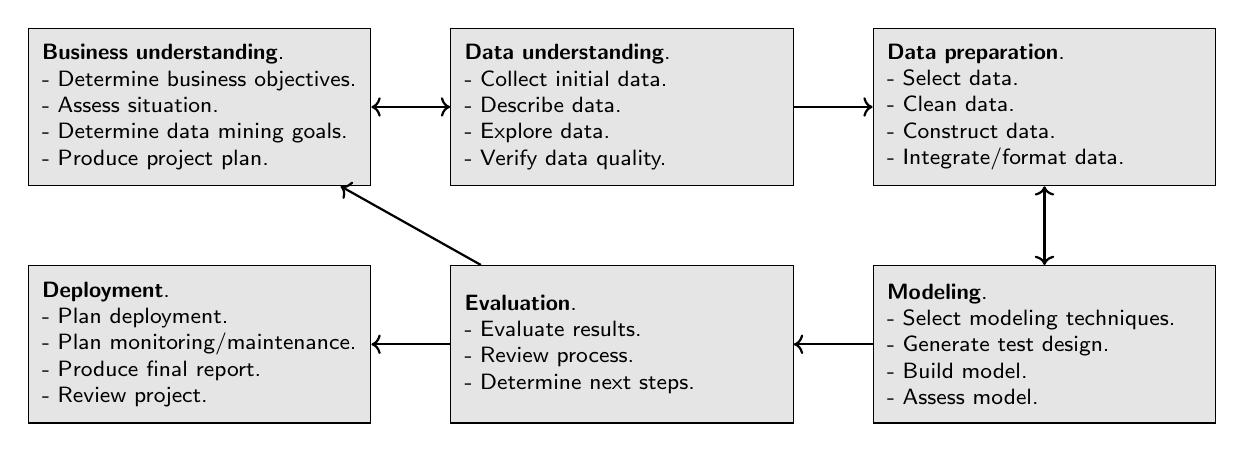
\begin{tikzpicture}
    [node distance = 2cm, auto,font=\footnotesize,
    % STYLES
    every node/.style={node distance=2cm},
    % The comment style is used to describe the characteristics of each force
    comment/.style={rectangle, inner sep= 5pt, text width=5cm, node distance=0.5cm, font=\scriptsize\sffamily},
    % The force style is used to draw the forces' name
    force/.style={rectangle, draw, fill=black!10, inner sep=5pt, text width=4cm, minimum height=2cm, font=\footnotesize\sffamily}]

    % Draw forces
    \node [force] (a) {
    \parbox{\linewidth}{
    \textbf{Business understanding}.\\
    - Determine business objectives.\\
    - Assess situation.\\
    - Determine data mining goals.\\
    - Produce project plan.
    }
    };
    \node [force, right=1cm of a] (b) {
    \parbox{\linewidth}{
    \textbf{Data understanding}.\\
    - Collect initial data.\\
    - Describe data.\\
    - Explore data.\\
    - Verify data quality.
    }
    };
    \node [force, right=1cm of b] (c) {
    \parbox{\linewidth}{
    \textbf{Data preparation}.\\
    - Select data.\\
    - Clean data.\\
    - Construct data.\\
    - Integrate/format data.
    }
    };
    \node [force, below=1cm of c] (d) {
    \parbox{\linewidth}{
    \textbf{Modeling}.\\
    - Select modeling techniques.\\
    - Generate test design.\\
    - Build model.\\
    - Assess model.
    }
    };
    \node [force, below=1cm of a] (e) {
    \parbox{\linewidth}{
    \textbf{Deployment}.\\
    - Plan deployment.\\
    - Plan monitoring/maintenance.\\
    - Produce final report.\\
    - Review project.
    }
    };
    \node [force, below=1cm of b] (f) {
    \parbox{\linewidth}{
    \textbf{Evaluation}.\\
    - Evaluate results.\\
    - Review process.\\
    - Determine next steps.
    }
    };

    \path[->,thick]
    (b) edge (c)
    (d) edge (f)
    (f) edge (e)
    (f) edge (a);

    \path[<->,thick]
    (a) edge (b)
    (c) edge (d);
    \end{tikzpicture}
    \end{frame}
  }

  {
    \setbeamertemplate{footline}[frame number]
    \begin{frame}{Chapter I: A Multi-dimensional View of Data Mining.}
        \begin{itemize}
            \item Why data mining?
            \item What is data mining?
            \item \textbf{A multi-dimensional view of data mining.}
            \item What kind of data can be mined?
            \item What kinds of patterns can be mined?
            \item What technologies are used?
            \item What kinds of applications are targeted?
            \item Major issues in data mining.
            \item A brief history of data mining.
            \item Summary.
        \end{itemize}
    \end{frame}
  }

  {
    \setbeamertemplate{footline}[frame number]
    \begin{frame}{A Multidimensional View of Data Mining}
        \begin{itemize}
            \item \textbf{Data to be mined}:\\
                  \small{Database data (extended relational, object oriented, heterogeneous, legacy), data warehouse, transactional data, stream, spatiotemporal, time-series, sequence, text and web, multi-media, graphs.}
            \item \textbf{Knowledge to be mined (or data mining functions)}:\\
                  \begin{itemize}
                      \item Characterization, discrimination, association, classification, clustering, outlier analysis, etc.
                      \item Descriptive vs. predictive data mining.
                      \item Multiple/integrated functions and mining at multiple levels.
                  \end{itemize}
            \item \textbf{Techniques utilized}:\\
                  \small{Database, data warehouse (OLAP), machine learning, statistics, pattern recognition, visualization, high performance computing, etc.}
            \item \textbf{Applications adapted}:\\
                  \small{Retail, telecommunication, banking, fraud analysis, bio data mining, stock market analysis, text mining, web mining, etc.}
        \end{itemize}
    \end{frame}
  }

  {
    \setbeamertemplate{footline}[frame number]
    \begin{frame}{Chapter I: What Kind of Data can be Mined?}
        \begin{itemize}
            \item Why data mining?
            \item What is data mining?
            \item A multi-dimensional view of data mining.
            \item \textbf{What kind of data can be mined?}
            \item What kinds of patterns can be mined?
            \item What technologies are used?
            \item What kinds of applications are targeted?
            \item Major issues in data mining.
            \item A brief history of data mining.
            \item Summary.
        \end{itemize}
    \end{frame}
  }

  {
    \setbeamertemplate{footline}[frame number]
    \begin{frame}{Data Mining: On What Kinds of Data?}
        \begin{itemize}
            \item Database oriented data sets and applications:
            \begin{itemize}
                \item Relational database.
                \item Data warehouse.
                \item Transactional database.
            \end{itemize}
            \item Advanced data sets and advanced applications:
            \begin{itemize}
                \item Data streams and sensor data.
                \item Time series data, temporal data, sequence data (incl. biosequences).
                \item Structure data, graphs, social networks and multi-linked data.
                \item Object-relational databases.
                \item Heterogeneous databases and legacy databases.
                \item NoSQL databases.
                \item Spatial data and spatiotemporal data.
                \item Multimedia databases.
                \item Text databases.
                \item The world wide web.
            \end{itemize}
        \end{itemize}
    \end{frame}
  }

  {
    \setbeamertemplate{footline}[frame number]
    \begin{frame}{Chapter I: What Kinds of Patterns can be Mined?}
        \begin{itemize}
            \item Why data mining?
            \item What is data mining?
            \item A multi-dimensional view of data mining.
            \item What kind of data can be mined?
            \item \textbf{What kinds of patterns can be mined?}
            \item What technologies are used?
            \item What kinds of applications are targeted?
            \item Major issues in data mining.
            \item A brief history of data mining.
            \item Summary.
        \end{itemize}
    \end{frame}
  }

  {
    \setbeamertemplate{footline}[frame number]
    \begin{frame}{Data Mining Function: I. Generalization}
    \textbf{Information integration and data warehous construction:}
    \begin{itemize}
        \item Data cleaning.
        \item Transformation.
        \item Integration.
        \item Multidimensional modeling.
    \end{itemize}
    \textbf{Data cube technology:}
    \begin{itemize}
        \item Characterization (contrast data characteristics).\\
              E.g. dry vs. wet regions from numerical humidity values.
        \item Discrimination.
        \item Generalization.
        \item Summary.
    \end{itemize}
    \end{frame}
  }

  {
    \setbeamertemplate{footline}[frame number]
    \begin{frame}{Data Mining Function: II. Association and Correlation Analysis}
    \textbf{Frequent patterns or item sets:}\\
    What items are frequently purchased together in your supermarket.\\[0.5cm]

    \textbf{Association, correlation vs. causality:}\\
    A typical association rule: Diapers $\rightarrow$ Beer $[0.5\%,75\%]$ (support, confidence).\\
    Are strongly associated items also strongly correlated?\\[0.5cm]

    \textbf{How to mine such patterns and rules efficiently in large datasets?}\\
    \textbf{How to use such patterns for classification, clustering and other applications?}
    \end{frame}
  }

  {
    \setbeamertemplate{footline}[frame number]
    \begin{frame}{Data Mining Function: III. Classification}
    \textbf{Classification and (class-)label prediction:}\\
    Construct models (functions) based on training examples. \\
    Hence: "supervised".\\
    Describe and distinguish classes or concepts for future prediction.\\
    E.g. classify countries based on climate or classify cars based on gas mileage.\\
    Classifying something means to predict unknown class labels. \\[0.5cm]

    \textbf{Typical methods:}\\
    Decision trees, naive Bayesian classification, support-vector machines, neural networks, rule-based classification, pattern-based classification, logistic regression \ldots\\[0.5cm]

    \textbf{Typical applications:}\\
    Credit-card-fraud detection, direct marketing, classifying stars, diseases, web pages \ldots
    \end{frame}
  }

  {
    \setbeamertemplate{footline}[frame number]
    \begin{frame}{Data Mining Function: IV. Cluster Analysis}
    \textbf{Unsupervised learning:} I.e. class labels are unknown.\\
    \textbf{Group data:} I.e. cluster houses to find distribution patterns.\\[0.5cm]

    Principle:\\
    Maximize intra class similarity and minimize inter class similarity.\\[0.5cm]

    What is \textbf{similarity?}
    \end{frame}
  }

  {
    \setbeamertemplate{footline}[frame number]
    \begin{frame}{Data Mining Function: V. Outlier Analysis}
    \textbf{Outlier}: A data object that does not comply with the general behavior of the data.\\[0.5cm]

    Noise or exception?\\
    One person's garbage could be another person's treasure.\\[0.5cm]

    \textbf{Methods:}\\
    By-product of clustering or regression analysis \ldots \\
    Useful in fraud detection or rare-events analysis.
    \end{frame}
  }

  {
    \setbeamertemplate{footline}[frame number]
    \begin{frame}{Time and Ordering: Sequential Pattern, Trend and Evolution Analysis}
    \textbf{Sequence, trend, and evolution analysis}.\\
    \begin{itemize}
        \item Trend, time-series and deviation analysis. \\
              E.g., regression and value prediction (forecasting).
        \item Sequential-pattern mining.\\
              E.g. customers first buy digital camera, then buy large SD memory cards.
        \item Periodicity analysis.
        \item Motifs and biological-sequence analysis.\\
              Approximate and consecutive motifs.
        \item Similarity-based analysis.\\
        \item Mining data streams.\\
              Ordered, time-varying, potentially infinite (unbounded).
    \end{itemize}
    \end{frame}
  }

  {
    \setbeamertemplate{footline}[frame number]
    \begin{frame}{Structure and Network Analysis}
    \textbf{Graph mining}:\\
    Finding frequent subgraphs (e.g. chemical compounds), trees (XML), substructures (web fragments), information-network analysis.\\[0.2cm]

    \textbf{Social networks}:
    \begin{itemize}
        \item Social networks: Actors (objects, nodes) and relationships (edges).\\
              E.g., author networks in CS, terrorist networks.
        \item Multiple heterogeneous networks.\\
              A person could be in multiple information networks: friends, family, classmates \ldots
        \item Links carry a lot of semantical information: link mining.
    \end{itemize}

    \textbf{Web mining}:
    \begin{itemize}
        \item Web is a big information network: from PageRank to Google.
        \item Analysis of web information networks.
        \item Web community discovery, opinion mining, usage mining \ldots
    \end{itemize}
    \end{frame}
  }

  {
    \setbeamertemplate{footline}[frame number]
    \begin{frame}{Evaluation of Knowledge}
    \textbf{Is all mined knowledge interesting?}
    \begin{itemize}
        \item One can mine tremendous amounts of "patterns" and knowledge.
        \item Some may fit only certain dimension space (time, location \ldots).
        \item Some may not be representative, may be transient \ldots
    \end{itemize}

    \textbf{Evaluation of mined knowledge $\rightarrow$ directly mine only interesting knowledge?}
    \begin{itemize}
        \item Descriptive vs. predictive.
        \item Coverage.
        \item Typically vs. predictive.
        \item Accuracy.
        \item Timeliness.
        \item \ldots
    \end{itemize}
    \end{frame}
  }

  {
    \setbeamertemplate{footline}[frame number]
    \begin{frame}{Chapter I: What Technologies are Used?}
        \begin{itemize}
            \item Why data mining?
            \item What is data mining?
            \item A multi-dimensional view of data mining.
            \item What kind of data can be mined?
            \item What kinds of patterns can be mined?
            \item \textbf{What technologies are used?}
            \item What kinds of applications are targeted?
            \item Major issues in data mining.
            \item A brief history of data mining.
            \item Summary.
        \end{itemize}
    \end{frame}
  }

  {
    \setbeamertemplate{footline}[frame number]
    \begin{frame}{Data Mining: Confluence of Multiple Disciplines}
    \centering
    \resizebox{6.5cm}{6.5cm}{%
    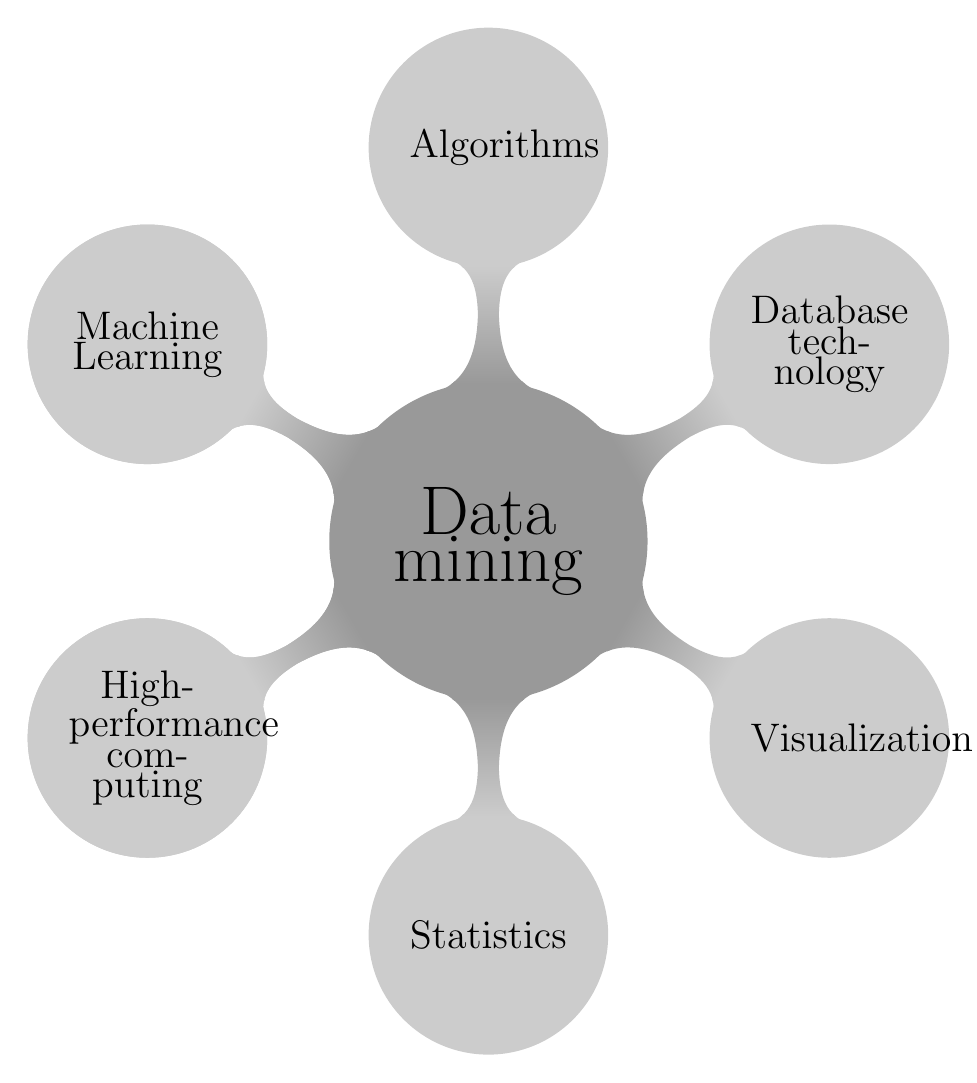
\begin{tikzpicture}[mindmap, minimum size=4cm, every node/.style=concept, concept color=black!40, grow cyclic]
        \node[concept] {\Huge Data mining}
        child [concept color=gray!40, minimum size=3cm]{node {\Large Machine Learning}}
        child [concept color=gray!40, minimum size=3cm]{node {\Large Pattern recognition}}
        child [concept color=gray!40, minimum size=3cm]{node {\Large Statistics}}
        child [concept color=gray!40, minimum size=3cm]{node {\Large Visualization}}
        child [concept color=gray!40, minimum size=3cm]{node {\Large Database technology}}
        child [concept color=gray!40, minimum size=3cm]{node {\Large Algorithms}}
        child [concept color=gray!40, minimum size=3cm]{node {\Large Machine Learning}}
        child [concept color=gray!40, minimum size=3cm]{node {\Large High-performance computing}};
    \end{tikzpicture}}
    \end{frame}
  }

  {
    \setbeamertemplate{footline}[frame number]
    \begin{frame}{Why Confluence of Multiple Disciplines?}
    \textbf{Tremendous amount of data:}
    \begin{itemize}
        \item Algorithms must be highly scalable to handle also terabytes of data.
    \end{itemize}

    \textbf{High dimensionality of data:}
    \begin{itemize}
        \item DNA microarrays may have tens of thousands of dimensions.\\
              Collections of microscopic DNA spots attached to a solid surface.
    \end{itemize}

    \textbf{High complexity of data:}
    \begin{itemize}
        \item Data streams and sensor data.
        \item Time-series data, temporal data, sequence data.
        \item Structure data, graphs, social networks, and multi-linked data.
        \item Heterogeneous databases and legacy databases.
        \item Spatial, spatiotemporal, multimedia, text and web data.
        \item Software programs, scientific simulations.
    \end{itemize}
    \textbf{New and sophisticated applications.}
    \end{frame}
  }

  {
    \setbeamertemplate{footline}[frame number]
    \begin{frame}{Chapter I: What Kinds of Applications are Targeted?}
        \begin{itemize}
            \item Why data mining?
            \item What is data mining?
            \item A multi-dimensional view of data mining.
            \item What kind of data can be mined?
            \item What kinds of patterns can be mined?
            \item What technologies are used?
            \item \textbf{What kinds of applications are targeted?}
            \item Major issues in data mining.
            \item A brief history of data mining.
            \item Summary.
        \end{itemize}
    \end{frame}
  }

  {
    \setbeamertemplate{footline}[frame number]
    \begin{frame}{Applications of Data Mining}
    \textbf{Web-page analysis:}\\
    From web-page classification, clustering to PageRank and HITS algorithms.\\
    HITS stands for Hyperlink-Induced Topic Search.\\[0.2cm]
    \textbf{Collaborative analysis and recommender systems.}\\
    \textbf{Basket-data analysis for targeted marketing.}\\
    \textbf{Biological and medical data analysis:}\\
    Classification, cluster analysis (microarray data analysis), biological sequence analysis, biological network analysis.\\[0.2cm]
    \textbf{Data mining and software engineering:}\\
    E.g. IEEE Computer, Aug. 2009 issue.\\
    \textbf{From major dedicated data mining systems/tools:}\\
    E.g. SAS, MS SQL-Server Analysis Manager, Oracle Data-Mining Tools.
    \end{frame}
  }

 {
    \setbeamertemplate{footline}[frame number]
    \begin{frame}{Chapter I: Major Issues in Data Mining.}
        \begin{itemize}
            \item Why data mining?
            \item What is data mining?
            \item A multi-dimensional view of data mining.
            \item What kind of data can be mined?
            \item What kinds of patterns can be mined?
            \item What technologies are used?
            \item What kinds of applications are targeted?
            \item \textbf{Major issues in data mining.}
            \item A brief history of data mining.
            \item Summary.
        \end{itemize}
    \end{frame}
  }

  {
    \setbeamertemplate{footline}[frame number]
    \begin{frame}{Major Issues in Data Mining (I)}
    \textbf{Mining methodology:}\\
    \begin{itemize}
        \item Mining various and new kinds of knowledge.
        \item Mining knowledge in multi-dimensional space.
        \item Data mining: An interdisciplinary effort.
        \item Boosting the power of discovery in a networked environment.
        \item Handling noise, uncertainty, and incompleteness of data.
        \item Pattern evaluation and pattern- or constraint-guided mining.
    \end{itemize}
    \textbf{User interaction:}\\
    \begin{itemize}
        \item Interactive mining.
        \item Incorporation of background knowledge.
        \item Presentation and visualization of data mining results.
    \end{itemize}
    \end{frame}
  }

  {
    \setbeamertemplate{footline}[frame number]
    \begin{frame}{Major Issues in Data Mining (II)}
    \textbf{Efficiency and scalability:}\\
    \begin{itemize}
        \item Efficiency and scalability of data-mining algorithms.
        \item Parallel, distributed, stream and incremental mining methods.
    \end{itemize}
    \textbf{Diversity of data types:}\\
    \begin{itemize}
        \item Handling complex types of data.
        \item Mining dynamic, networked and global data repositories.
    \end{itemize}
    \textbf{Data mining and society:}\\
    \begin{itemize}
        \item Social impacts of data mining.
        \item Privacy-preserving data mining.
        \item Invisible data mining.
    \end{itemize}
    \end{frame}
  }


 {
    \setbeamertemplate{footline}[frame number]
    \begin{frame}{Chapter I: A Brief History of Data Mining.}
        \begin{itemize}
            \item Why data mining?
            \item What is data mining?
            \item A multi-dimensional view of data mining.
            \item What kind of data can be mined?
            \item What kinds of patterns can be mined?
            \item What technologies are used?
            \item What kinds of applications are targeted?
            \item Major issues in data mining.
            \item \textbf{A brief history of data mining.}
            \item Summary.
        \end{itemize}
    \end{frame}
  }

 {
    \setbeamertemplate{footline}[frame number]
    \begin{frame}{A Brief History of Data Mining Society}
        \begin{itemize}
            \item \textbf{1989 IJCAI Workshop on Knowledge Discovery in Databases:}\\
                  Knowledge Discovery in Databases (G. Piatetsky-Shapiro and W. Frawley, 1991).
            \item \textbf{1991-1994 Workshops on Knowledge Discovery in Databases:}\\
                  Advances in Knowledge Discovery and Data Mining (U. Fayyad, G. Piatetsky-Shapiro, P. Smyth and R. Uthurusamy, 1996).
            \item \textbf{1995-1998 International Conferences on Knowledge Discovery in Databases and Data Mining (KDD’95-98):}\\
                  Journal of Data Mining and Knowledge Discovery (1997).
            \item \textbf{ACM SIGKDD conferences since 1998 and SIGKDD Explorations.}\\
            \item \textbf{More conferences on data mining:}\\
                  PAKDD (1997), PKDD (1997), SIAM-Data Mining (2001), (IEEE) ICDM (2001), etc.
            \item \textbf{Journal ACM Transactions on KDD starting in 2007}.
        \end{itemize}
    \end{frame}
  }

  {
    \setbeamertemplate{footline}[frame number]
    \begin{frame}{Conferences and Journals on Data Mining (I)}
    \textbf{KDD Conferences:}
        \begin{itemize}
            \item ACM SIGKDD Int. Conf. on Knowledge Discovery in Databases and Data Mining (KDD).
            \item SIAM Data Mining Conf. (SDM).
            \item (IEEE) Int. Conf. on Data Mining (ICDM).
            \item European Conf. on Machine Learning and Principles and Practices of Knowledge Discovery and Data Mining (ECML-PKDD).
            \item Pacific-Asia Conf. on Knowledge Discovery and Data Mining (PAKDD).
            \item Int. Conf. on Web Search and Data Mining (WSDM).
        \end{itemize}
    \end{frame}
  }

  {
    \setbeamertemplate{footline}[frame number]
    \begin{frame}{Conferences and Journals on Data Mining (II)}
    \textbf{Other related conferences:}
        \begin{itemize}
            \item DB conferences: ACM SIGMOD, VLDB, ICDE, EDBT, ICDT, \ldots
            \item Web and IR conferences: WWW, SIGIR, WSDM, \ldots
            \item ML conferences: ICML, NIPS, ICLR \ldots
            \item PR conferences: CVPR, ICPR \ldots
        \end{itemize}
    \textbf{Journals:}
        \begin{itemize}
            \item Data Mining and Knowledge Discovery (DAMI or DMKD).
            \item IEEE Trans. On Knowledge and Data Eng. (TKDE).
            \item KDD Explorations.
            \item ACM Trans. on KDD.
        \end{itemize}
    \end{frame}
  }

  {
    \setbeamertemplate{footline}[frame number]
    \begin{frame}{Where to Find References? DBLP, CiteSeer, Google (I)}
    \textbf{Data mining and KDD (SIGKDD: CD-ROM):}
        \begin{itemize}
            \item Conferences: ACM-SIGKDD, IEEE-ICDM, SIAM-DM, PKDD, PAKDD, etc.
            \item Journal: Data Mining and Knowledge Discovery, KDD Explorations, ACM TKDD.
            \item KDnuggets: \url{www.kdnuggets.com}.
        \end{itemize}
    \textbf{Database systems (SIGMOD: ACM SIGMOD Anthology CD-ROM):}
        \begin{itemize}
            \item Conferences: ACM-SIGMOD, ACM-PODS, VLDB, IEEE-ICDE, EDBT, ICDT, DASFAA.
            \item Journals: IEEE-TKDE, ACM-TODS/TOIS, JIIS, J. ACM, VLDB J., Info. Sys., etc.
        \end{itemize}
    \textbf{AI \& Machine Learning:}
        \begin{itemize}
            \item Conferences: Machine learning (ML), AAAI, IJCAI, COLT (Learning Theory), CVPR, NIPS, etc.
            \item Journals: Machine Learning, Artificial Intelligence, Knowledge and Information Systems, IEEE-PAMI, etc.
        \end{itemize}
    \end{frame}
  }

  {
    \setbeamertemplate{footline}[frame number]
    \begin{frame}{Where to Find References? DBLP, CiteSeer, Google (II)}
    \textbf{Web and IR:}
        \begin{itemize}
            \item Conferences: SIGIR, WWW, CIKM, etc.
            \item Journals: WWW: Internet and Web Information Systems.
        \end{itemize}
    \textbf{Statistics:}
        \begin{itemize}
            \item Conferences: Joint Stat. Meeting, etc.
            \item Journals: Annals of Statistics, etc.
        \end{itemize}
    \textbf{Visualization:}
        \begin{itemize}
            \item Conferences: CHI, ACM-SIGGraph, etc.
            \item Journals: IEEE Trans. Visualization and Computer Graphics, etc.
        \end{itemize}
    \end{frame}
  }

 {
    \setbeamertemplate{footline}[frame number]
    \begin{frame}{Chapter I: Summary.}
        \begin{itemize}
            \item Why data mining?
            \item What is data mining?
            \item A multi-dimensional view of data mining.
            \item What kind of data can be mined?
            \item What kinds of patterns can be mined?
            \item What technologies are used?
            \item What kinds of applications are targeted?
            \item Major issues in data mining.
            \item A brief history of data mining.
            \item \textbf{Summary.}
        \end{itemize}
    \end{frame}
  }

 {
    \setbeamertemplate{footline}[frame number]
    \begin{frame}{Summary}
    \textbf{Data mining:}\\
    Discovering interesting patterns and knowledge from massive amounts of data.\\[0.2cm]

    \textbf{A natural evolution of database technology:}\\
    In great demand, with wide applications.\\[0.2cm]

    \textbf{KDD pipeline includes:}\\
    Data cleaning, data integration, data selection, transformation, data mining, pattern evaluation and knowledge presentation.\\[0.2cm]

    \textbf{Mining can be performed in a variety of data.}\\
    \textbf{Data-mining functionalities:}\\
    Characterization, discrimination, association, classification, clustering, outlier and trend analysis, etc.\\[0.2cm]

    \textbf{Data-mining technologies and applications.}\\
    \textbf{Major issues in data mining.}\\
    \end{frame}
  }


  {
    \setbeamertemplate{footline}[frame number]
    \begin{frame}{References (I)}
        \begin{itemize}
          \item S. Chakrabarti: \emph{Mining the Web: Statistical Analysis of Hypertext and Semi-Structured Data}. Morgan Kaufmann, 2002.
          \item T. Dasu and T. Johnson: \emph{Exploratory Data Mining and Data Cleaning}. John Wiley \& Sons, 2003.
          \item R. Duda, P. E. Hart and D. Stork: \emph{Pattern Classification}. 2ed., Wiley-Interscience, 2000.
          \item U. Fayyad, G. Piatetsky-Shapiro, P. Smyth and R. Uthurusamy: \emph{Advances in Knowledge Discovery and Data Mining}. AAAI/MIT Press, 1996.
          \item U. Fayyad, G. Grinstein and A. Wierse: \emph{Information Visualization in Data Mining and Knowledge Discovery}, Morgan Kaufmann, 2001.
          \item J. Han, M. Kamber and J. Pei: \emph{Data Mining: Concepts and Techniques}. Morgan Kaufmann, 3rd ed., 2012.
          \item D. Hand, H. Mannila and P. Smyth: \emph{Principles of Data Mining}. MIT Press, 2001.
          \item T. Hastie, R. Tibshirani and J. Friedman: \emph{The Elements of Statistical Learning: Data Mining, Inference, and Prediction}. 2nd ed., Springer-Verlag, 2009.
        \end{itemize}
    \end{frame}
  }

  {
    \setbeamertemplate{footline}[frame number]
    \begin{frame}{References (II)}
        \begin{itemize}
          \item B. Liu: \emph{Web Data Mining}. Springer 2006.
          \item T. M. Mitchell: \emph{Machine Learning}. McGraw Hill, 1997.
          \item G. Piatetsky-Shapiro and W. Frawley: \emph{Knowledge Discovery in Databases}. AAAI/MIT Press, 1991.
          \item P.-N. Tan, M. Steinbach and V. Kumar: \emph{Introduction to Data Mining}. Wiley, 2005.
          \item S. M. Weiss and N. Indurkhya: \emph{Predictive Data Mining}. Morgan Kaufmann, 1998.
          \item I. H. Witten, E. Frank and M. A. Hall: \emph{Data Mining: Practical Machine Learning Tools and Techniques}. Morgan Kaufmann, 3rd ed. 2011.
          \item C. Shearer: \emph{The CRISP-DM Model: The New Blueprint for Data Mining}. Journal of Data Warehousing, vol. 5, no. 4, pp. 13-22.
          \item T. Xie, S. Thummalapenta, D. Lo and C. Liu: \emph{Data Mining for Software Engineering}. IEEE Computer, August 2009, pp. 55-62.
          \item R. Hyndman and G. Athanasopoulos: \emph{Forecasting: Principles and Practice}. 2nd ed. Monash University, Australia, April 2018.
        \end{itemize}
    \end{frame}
  }


  { % Questions?
    \setbeamertemplate{footline}[frame number]
    \begin{frame}[c]
      \begin{center}
        Thank you for your attention.\\
        {\bf Any questions about the first chapter?}\\[0.5cm]
        Ask them now, or again, drop me a line: \\
        \faSendO \ \texttt{luciano.melodia@fau.de}.
      \end{center}
    \end{frame}
  }
\end{document}
